% Tex root = ../main.tex

\subsection{Modelado del motor en el espacio de estados}
El primer paso en el modelado del motor es analizar el comportamiento de
los componentes de interés. En este caso se considerará como entrada el
voltaje de entrada del motor ($V_{in}$), y como salida la velocidad
angular de la flecha ($\omega_m$).
Las variables de estado serán la corriente del sistema ($I_t$),
la posición angular ($\theta$) y la velocidad angular ($\omega_m$).
Tal como se muestra en la figura \ref{fig:Motor-LTI-CajaNegra}.
\begin{figure}[H]
  \begin{center}
    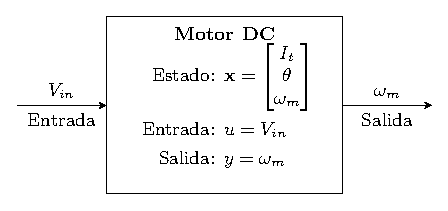
\includegraphics[width=0.98\linewidth]{img.tex-svg/Motor-LTI-CajaNegra.pdf}
    \caption{Esquema de caja negra con las variables de entrada, estado
    y salida del sistema modelado.}
    \label{fig:Motor-LTI-CajaNegra}
  \end{center}
\end{figure}

El modelo en espacio de estados se, tal como se muestra en el sistema
de ecuaciones \eqref{eq:EspacioEstados}.
\begin{equation}
  \label{eq:EspacioEstados}
  \begin{cases}
    \dot{\mathbf{x}} &= \mathbf{A} \mathbf{x} + \mathbf{B} u \\
    y &= \mathbf{C} \mathbf{x} + \mathbf{D} u
  \end{cases}
\end{equation}

\subsubsection{Análisis del voltaje en el rotor}

Para el análisis del sistema, se consideraron los voltajes para realizar
el modelado.

\begin{equation}
  \label{eq:Motor-LTI-Modelo}
  \begin{cases}
    V_r    &= iR  \\
    V_{L_r}&=L \frac{di}{dt}
  \end{cases}
\end{equation}

Donde i, representa a la corriente total del sistema.

También existe un voltaje negativo que se opone al voltaje de entrada:
la fuerza contraelectromotriz $V_M$, que se obtiene como efecto del proceso
electromagnético que ocurre dentro del motor.

Esta fuerza se vincula directamente con la velocidad angular de la flecha

$$V_{M} = K_e \omega_m$$

donde $K_e$ es la constante electromotriz.

Teniendo en cuenta estos elementos, es posible realizar el análisis de voltajes
en el rotor de un motor de DC.

\begin{equation*}
  \begin{cases}
    V_r    &= iR  \\
    V_{L_r}&=L \frac{di}{dt} \\
    V_{M}  &= K_e \omega_m
  \end{cases}
\end{equation*}
Y debido a que
$$
\sum_i V_i = 0
$$
Tenemos que los voltajes se relacionan de la forma
\begin{equation}
  \begin{aligned}
    -V_{in} + V_r + V_{L_r}       + V_{M} &= 0\\
    -V_{in} + Ri  + L\frac{di}{dt} + K_e\omega_m &= 0
  \end{aligned}
\end{equation}

De esta ecuación nos interesa el comportamiento de la corriente en el tiempo.
\begin{equation*}
  \begin{aligned}
    \frac1L \left(
      -V_{in} + Ri  + L\frac{di}{dt} + K_e\omega_m
    \right) &=\frac1L  (0) \\
      -\frac{V_{in}}L + \frac{Ri}L  + \frac{di}{dt} + \frac{K_e\omega_m}{L}
     &=  0 \\
  \end{aligned}
\end{equation*}
Obteniendo la siguiente ecuación diferencial
\begin{equation}
      \frac{di}{dt} = \frac{V_{in}}L - \frac{Ri}L  - \frac{K_e\omega_m}{L}
      \label{eq:DiferencialCorriente}
\end{equation}

Nuestras funciones en el espacio de estados se describen a partir de la
matriz

\subsubsection{Análisis mecánico del motor}
Al ser este tipo de sistemas un transformador (eléctrico-mecánico), se
necesita también conocer el comportamiento de la sección mecánica.

El par motriz $\tau_m$ es directamente proporcional al toque $K_t$ y la corriente
total de sistema $i$. El par de fricción viscoso $\tau_f$ es proporcional a
la velocidad angular $\omega_m$ y el coeficiente de fricción viscoso $B$.

\begin{equation*}
  \begin{cases}
    \tau_m = K_t i\\
    \tau_f = B \omega_m
  \end{cases}
\end{equation*}

De este modo, podemos a partir el esfuerzo de aceleración del motor $J$
podemos obtener la ecuación diferencial de la velocidad angular
\eqref{eq:DiferencialVelocidadAngular}.

\begin{equation*}
  \begin{aligned}
    J\frac{d\omega_m}{dt} &= \tau_m - \tau_f\\
   \frac1J  \left(
      J\frac{d\omega_m}{dt}
    \right)
   &=
   \frac1J  \left(
      \tau_m - \tau_f
    \right)\\
  \end{aligned}
\end{equation*}

\begin{equation}
  \frac{d\omega_m}{dt} = \frac{K_t i - B \omega_m}{J}\\
  \label{eq:DiferencialVelocidadAngular}
\end{equation}


\subsubsection{Matrices del sistema en el espacio de estados}
Es apreciable que las ecuaciones \eqref{eq:DiferencialCorriente} y
\eqref{eq:DiferencialVelocidadAngular} se puede obtener el
vector de ecuaciones diferenciales
$\dot{\mathbf{x}}$ de la forma

\begin{equation}
  \begin{cases}
    \dot{\mathbf{x}}&=\begin{bmatrix}
     -\frac{R}{L}   & 0 & -\frac{K_e}{L} \\
      0             & 0 &   1            \\
      \frac{K_t}{J} & 0 & -\frac{B}{J}   \\
    \end{bmatrix}
    \begin{bmatrix}
      I_t\\ \theta\\ \omega_m
    \end{bmatrix}
    +\begin{bmatrix} 
      \frac{1}{L} \\
      0\\
      0\\
    \end{bmatrix} u\\
    y &= \begin{bmatrix}
      0 & 0 & 1\\
    \end{bmatrix}
    \begin{bmatrix}
      I_t\\ \theta\\ \omega_m
    \end{bmatrix}
  \end{cases}
\end{equation}

De aquí es evidente que la posición angular no tiene efecto sobre
nuestra salida que es la velocidad angular.
Las matrices que obtenemos después del análisis se pueden apreciar
en la ecuación \eqref{eq:MatricesEspacioEstados}

\begin{equation}
  \begin{aligned}
    \mathbf{A} &= \begin{bmatrix}
    -\frac{R}{L}  & 0 & -\frac{K_e}{L} \\
    0             & 0 &  1           \\
    \frac{K_t}{J} & 0 & -\frac{B}{J} \\
  \end{bmatrix} &
    \mathbf{B} &= \begin{bmatrix}
    \frac{1}{L} \\
    0\\
    0\\
  \end{bmatrix} \\
  \mathbf{C} &= \begin{bmatrix}
      0 & 0 & 1
    \end{bmatrix} &
    \mathbf{D} &= 0
 \end{aligned}
  \label{eq:MatricesEspacioEstados}
\end{equation}
